\onecolumn
\chapter{Auswertung}
% Liste der genutzer Formeln für die Fehlerrechnung
\section*{Fehlerrechnung}
Für die statistische Auswertung von $n$ Messwerten $x_i$ werden folgende Größen definiert \cite{errorSkript25}:
\begin{align}
    \bar{x} &= \frac{1}{n} \sum_{i=1}^{n} x_i \vphantom{\sqrt{\sum_i^n}^2} && \text{\textcolor{gray}{Arithmetisches Mittel}} \label{eq:arithmetisches_mittel} \\
    \sigma^2 &= \frac{1}{n-1} \sum_{i=1}^{n} (x_i - \bar{x})^2 \vphantom{\sqrt{\sum_i^n}^2} && \text{\textcolor{gray}{Variation}} \label{eq:variation} \\
    \sigma &= \sqrt{\frac{1}{n-1} \sum_{i=1}^{n} (x_i - \bar{x})^2} \vphantom{\sqrt{\sum_i^n}^2} && \text{\textcolor{gray}{Standardabweichung}} \label{eq:standardabweichung} \\
    \Delta \bar{x} &= \frac{\sigma}{\sqrt{n}} = \sqrt{\frac{1}{n(n-1)} \sum_{i=1}^n(\bar x - x_i)^2} \vphantom{\sqrt{\sum_i^n}^2} && \text{\textcolor{gray}{Fehler des Mittelwerts}} \label{eq:fehler_mittelwert} \\
    \Delta f &= \sqrt{\left(\frac{\partial f}{\partial x} \Delta x\right)^2 + \left(\frac{\partial f}{\partial y} \Delta y\right)^2} \vphantom{\sqrt{\sum_i^n}^2} && \text{\textcolor{gray}{Gauß’sches Fehlerfortpflanzungsgesetz für $f(x,y)$}} \label{eq:gauss_fehlfortpflanzung} \\
    \Delta f &= \sqrt{(\Delta x)^2 + (\Delta y)^2} \vphantom{\sqrt{\sum_i^n}^2} && \text{\textcolor{gray}{Fehler für $f = x + y$}} \label{eq:fehler_summe} \\
    \Delta f &= |a| \Delta x \vphantom{\sqrt{\sum_i^n}^2} && \text{\textcolor{gray}{Fehler für $f = ax$}} \label{eq:fehler_proportional} \\
    \frac{\Delta f}{|f|} &= \sqrt{\left(\frac{\Delta x}{x}\right)^2 + \left(\frac{\Delta y}{y}\right)^2} \vphantom{\sqrt{\sum_i^n}^2} && \text{\textcolor{gray}{relativer Fehler für $f = xy$ oder $f = x/y$}} \label{eq:relativer_fehler} \\
    \sigma &= \frac{|a_{lit} - a_{gem}|}{\sqrt{\Delta a_{lit}^2 + \Delta a_{gem}^2}} \vphantom{\sqrt{\sum_i^n}^2} && \text{\textcolor{gray}{Berechnung der signifikanten Abweichung}} \label{eq:signifikante_abweichung}
\end{align}

\twocolumn

\section{Fehlerbestimmung zweier Messmethoden}
Zunächst werden die beiden Methoden unabhänig voneinander ausgewertet und die Ergebnisse miteinander verglichen. Ziel ist es, die Methode mit der geringeren Unsicherheit zu identifizieren und diese für die weiteren Messungen zu verwenden.
\subsection*{Methode 1}
Wir schauen uns zunächst die erste Methode an, bei der die Periodendauer $T_{m}$ über die maximale Auslenkung des Pendels gemessen wird. Die Messwerte sind aus dem Protokoll \ref{Protokoll} entnommen. Die in Tabelle \ref{tab:max_Auslenkung} aufgelisteten Werte sind auf die Wesentlichen beschrängt.
Dabei ist $T_{m}$ die gemessene Periodendauer, $\Delta T_{m}$ der absolute Fehler und $\Delta T_{m} (\%)$ der relative Fehler in Prozent.
\messwertetabelle

\begin{figure}[h!]
    \centering
    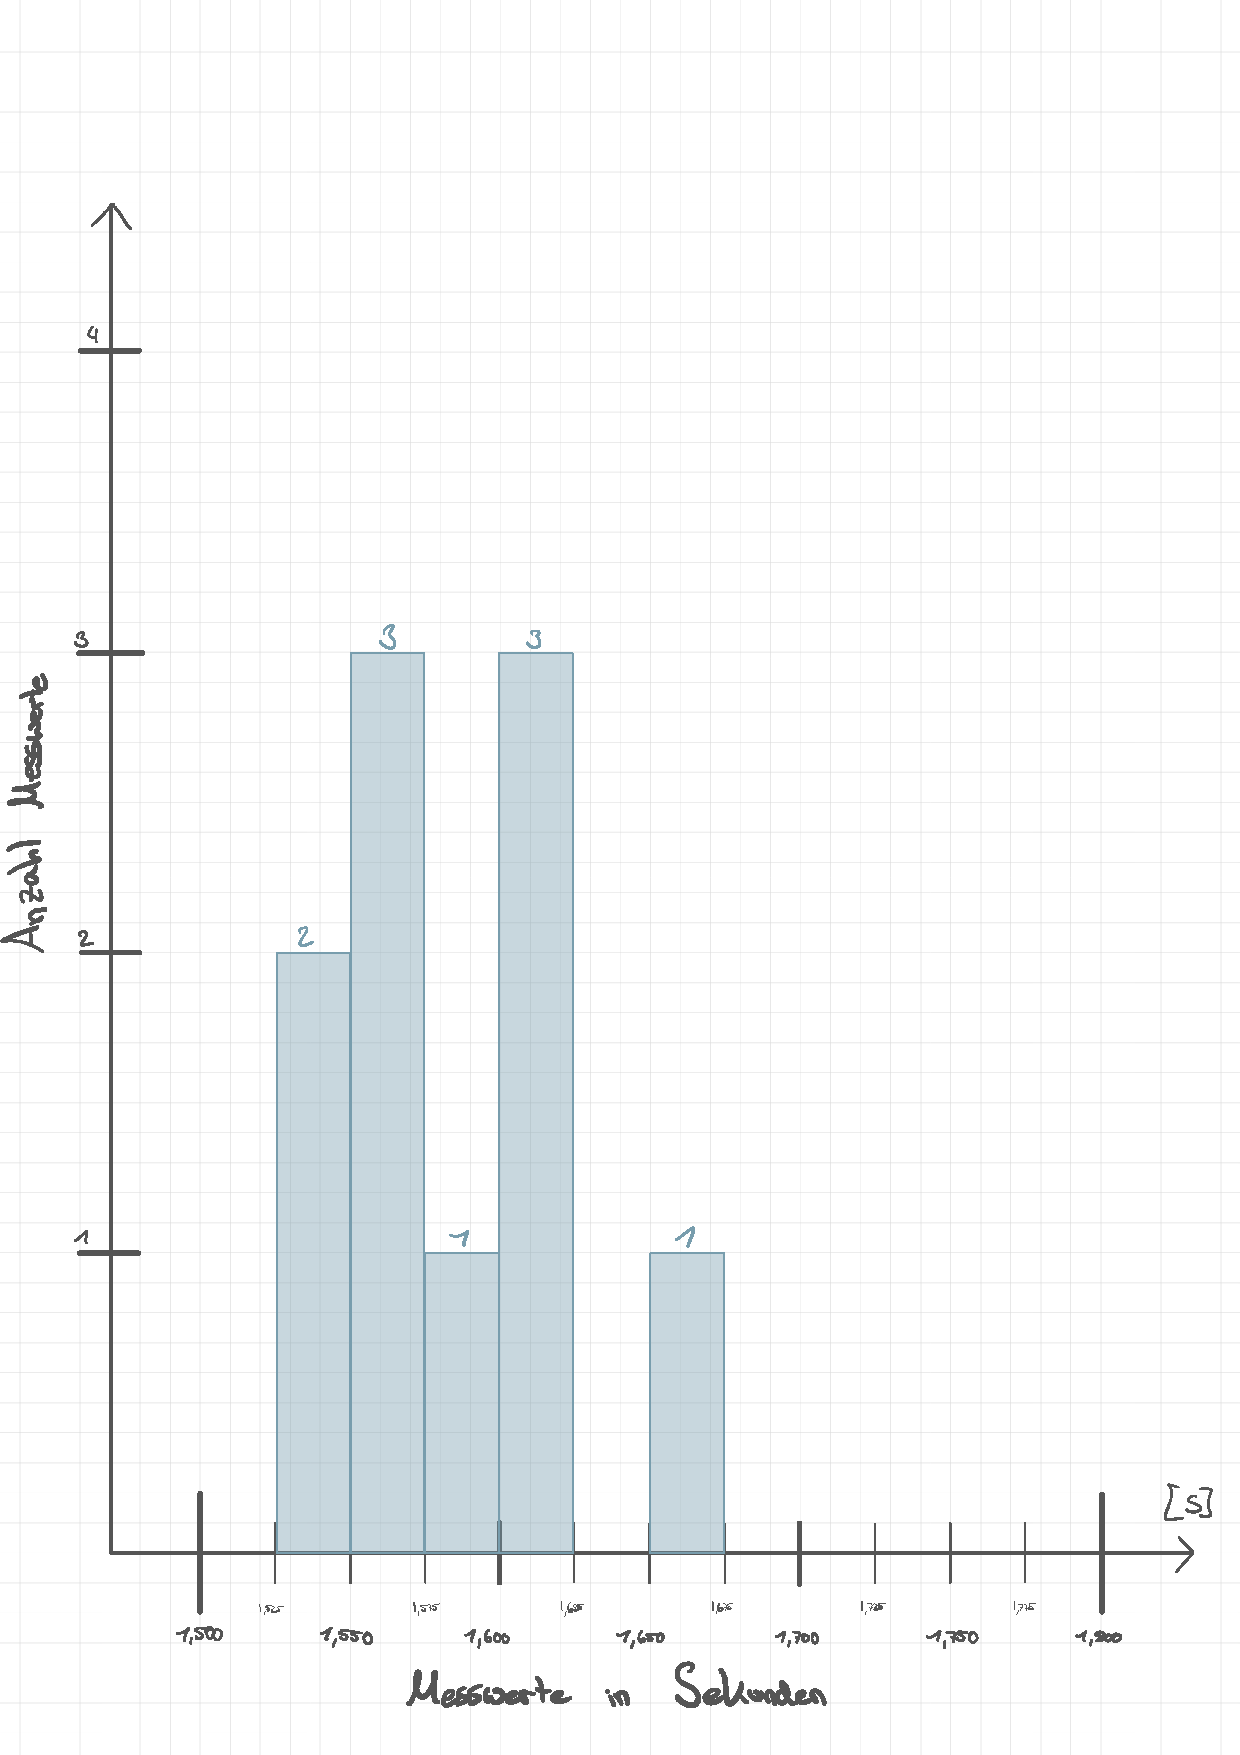
\includegraphics[width=0.45\textwidth, page=1]{img/\versuchsnummer/11-Graphen.pdf}
    \caption{Histogramm der Messwerte bei maximaler Auslenkung des Pendels}
    \label{fig:histogramm_max_auslenkung}
\end{figure}



\vspace{2pt}
Der Mittelwert \eqref{eq:arithmetisches_mittel} der Periodendauer beträgt:
\begin{equation}
    \bar{T}_{m} = \frac{1}{\anzahlmesswerte}\sum_{i=1}^{\anzahlmesswerte} T_{m,i} = \underline{\mittelwert\,\mathrm{s}}.
\end{equation}
Über diesen Mittelwert  sind auch die Abweichungen der Einzelwerte $\Delta T$ berechnet.

Der mittlere Fehler des Mittelwerts \eqref{eq:fehler_mittelwert} berechnet sich zu:
\begin{align}
    \Delta \bar{T}_{m} &= \sqrt{\frac{1}{10(10-1)} \sum_{i=1}^{10} (\bar{x}-x_i)^2}  \\
    \Delta \bar{T}_{m} &= \underline{\statistischerfehler\,\mathrm{s}}
\end{align}

Wir kommen also zu dem Ergebnis:
\begin{equation}
    \underline{\underline{T_{m} = \bar{T}_{m} \pm \Delta \bar{T}_{m} = (1,587 \pm 0,014)\,\mathrm{s}.}}
\end{equation}

\subsection*{Methode 2}
Nun vergleichen wir das mit der zweiten Methode, bei der die Periodendauer $T_{n}$ über den Nulldurchgang des Pendels gemessen wird. Die Messwerte sind aus dem Protokoll \ref{Protokoll} entnommen. Die in Tabelle \ref{tab:null_Auslenkung} aufgelisteten Werte sind auf die Wesentlichen beschrängt.
\begin{table}[h!]
\centering

\begin{tabular}{c|c|c|c}
Messung & $T_{n} [s]$ & $\Delta T_{n} [s]$ & $\Delta T_{n} [\%]$ \\
\hline
1 & 1,687 & -0,002 & -0,12 \\
2 & 1,713 & 0,024 & 1,42 \\
3 & 1,697 & 0,008 & 0,47 \\
4 & 1,713 & 0,024 & 1,42 \\
5 & 1,713 & 0,024 & 1,42 \\
6 & 1,697 & 0,008 & 0,47 \\
7 & 1,643 & -0,046 & -2,72 \\
8 & 1,687 & -0,002 & -0,12 \\
9 & 1,673 & -0,016 & -0,95 \\
10 & 1,667 & -0,022 & -1,30 \\
\hline
$\bar{T}_{n}$ & 1,689 & & \\
\end{tabular}
\caption{Periodendauer berechnet durch die Messung bei Nullauslenkung des Pendels}
\label{tab:null_Auslenkung}
\end{table}

\begin{figure}[h!]
    \centering
    \includegraphics[width=0.45\textwidth, page=2]{img/\versuchsnummer/11-Graphen.pdf}
    \caption{Histogramm der Messwerte bei Nulldurchgang des Pendels}
    \label{fig:histogramm_null_auslenkung}
\end{figure}


Der Mittelwert \eqref{eq:arithmetisches_mittel} der Periodendauer beträgt:
\begin{equation}
    \bar{T}_{n} = \frac{1}{\anzahlmesswerte}\sum_{i=1}^{\anzahlmesswerte} T_{n,i} = \underline{1,689\,\mathrm{s}}.
\end{equation}
Über diesen Mittelwert sind wieder die Abweichungen der Einzelwerte $\Delta T_{n}$ berechnet.
Der mittlere Fehler des Mittelwerts \eqref{eq:fehler_mittelwert} berechnet sich zu:
\begin{align}
    \Delta \bar{T}_{n} & = \sqrt{\frac{1}{10(10-1)} \sum_{i=1}^{10} (\bar{x}-x_i)^2} \\
    \Delta \bar{T}_{n} & = \underline{0,096\,\mathrm{s}}.
\end{align}

Für die zweite Methode ergibt sich somit:
\begin{equation}
    \underline{\underline{T_{n} = \bar{T}_{n} \pm \Delta \bar{T}_{n} = (1,690 \pm 0,010)\,\mathrm{s}.}} 
\end{equation}

\subsection*{Vergleich der Methoden}
Nun können wir die beiden Methoden miteinander vergleichen. Die erste Methode liefert eine Periodendauer von $T_{m} = (1,587 \pm 0,014)\,\mathrm{s}$, während die zweite Methode eine Periodendauer von $T_{n} = (1,689 \pm 0,096)\,\mathrm{s}$ ergibt.
Über die Werte bestimmen wir nun die Standardabweichung \eqref{eq:standardabweichung} des Mittelwertes. Die kleinere Standardabweichung deutet auf die genauere Methode hin:
\begin{align}
    \sigma_{\bar{T}_m} &= \sqrt{\frac{1}{9} \sum_{i=1}^{10} (\bar{T_m}-T_{m,i})^2} = \underline{0,043\,\mathrm{s}} \\
    \sigma_{\bar{T}_n} &= \sqrt{\frac{1}{9} \sum_{i=1}^{10} (\bar{T_n}-T_{n,i})^2} = \underline{0,030\,\mathrm{s}}
\end{align}

Eindeutig zusehen ist, dass Methode 2, also die Messung über den \emph{Nulldurchgang} die kleinere Standardabweichung aufweist und somit die genauere Methode ist. Diese wird im Folgenden für die weiteren Messungen verwendet.

\begin{figure}[h!]
    \centering
    \includegraphics[width=0.45\textwidth, page=3]{img/\versuchsnummer/11-Graphen.pdf}
    \caption{Überlagerung der beiden Histogramme zur besseren Vergleichbarkeit}
    \label{fig:histogramm_vergleich}
\end{figure}

\section{Messen der Schwingungsdauer als Funktion der Masse}
Nun geht es zum nächsten Schritt: die Abhängigkeit der Schwingungsdauer $T$ von der angehängten Masse $m$ zu untersuchen. Die Messwerte sind aus dem Protokoll \ref{Protokoll} entnommen. Die in Tabelle \ref{tab:verschiedene_massen_messungen} aufgelisteten Werte sind auf die Wesentlichen beschrängt.
Das Ziel ist es eine Funktion in Abhängigkeit der Federkonstante $D$ zu bestimmen.

\begin{table}[h!]
    \centering
    \begin{tabular}{c | c | c | c}
    Masse [g] & $T$ [s] & $\bar{T}$ [s] & $\Delta \bar{T}$ [s] \\
    \hline
    50  & 0,927 & 0,933 & 0,004 \\
        & 0,933 &       &       \\
        & 0,940 &       &       \\
    \hline
    100 & 1,213 & 1,218 & 0,004 \\
        & 1,213 &       &       \\
        & 1,227 &       &       \\
    \hline
    150 & 1,500 & 1,501 & 0,005 \\
        & 1,510 &       &       \\
        & 1,493 &       &       \\
    \hline
    200 & 1,673 & 1,680 & 0,014 \\
        & 1,707 &       &       \\
        & 1,660 &       &       \\
    \hline
    250 & 1,863 & 1,860 & 0,007 \\
        & 1,870 &       &       \\
        & 1,847 &       &       \\
    \hline
    \end{tabular}
    \caption{Messungen der Pendelperioden bei verschiedenen Massen}
    \label{tab:verschiedene_massen_messungen}
\end{table}

Zu Berechnung der Federkonstante $D$ wird die Formel für die Periodendauer \eqref{eq:periodendauer} eines Federpendels verwendet und umgeschrieben in:
\begin{equation}
    T^2 = \frac{4 \pi^2}{D} \cdot m.
    \label{eq:periodendauer_umgestellt}
\end{equation}

Diese Gleichung kann man als Geradengleichung der Form $y = ax + b$ interpretieren, wobei:
\begin{align}
    y &= T^2 \\
    x &= m \\
    a &= \frac{4 \pi^2}{D} \\
    b &= 0
\end{align}
ist. natürlich sind unsere Werte mit Ungenauigkeiten behaftet.
Daher nutzen wir das Fehlerfortpflanzungsgesetz \eqref{eq:gauss_fehlfortpflanzung}, um die Unsicherheiten zu bestimmen:
\begin{equation}
    \Delta \bar{T}^2 = 2 \bar{T} \cdot \Delta \bar{T}
\end{equation}

Um eine bessere übersicht zu gewinnen, sortieren wir Tabelle \ref{tab:verschiedene_massen_messungen} um und berechnen $\bar{T}^2$ und die jeweiligen Unsicherheiten $\Delta \bar{T}^2$.
\begin{table}[h!]
    \centering
    \begin{tabular}{c | c | c | c | c}
    Masse [g] & $\bar{T} [s]$  & $\Delta \bar{T} [s]$ & $\bar{T}^2 [s^2]$ & $\Delta \bar{T}^2$ [s$^2$] \\
    \hline
    50  & 0,933 & 0,004 & 0,870 & 0,007\\
    100 & 1,218 & 0,004 & 1,484 & 0,010\\
    150 & 1,501 & 0,005 & 2,253 & 0,015\\
    200 & 1,680 & 0,014 & 2,822 & 0,047\\
    250 & 1,860 & 0,007 & 3,460 & 0,026\\
    \hline
    \end{tabular}
    \caption{Berechnete Werte für $T^2$ und die Unsicherheiten}
    \label{tab:berechnete_werte}
\end{table}

Die Unsicherheit der Masse wird als nicht relevant angenommen, ist aber sehr wohl existent.
Somit können wir die Gleichung \eqref{eq:periodendauer_umgestellt} umstellen, sodass wir die steigung berechnen können.
\begin{equation}
    \frac{\Delta T^2}{\Delta m} = a
    \label{eq:steigung}
\end{equation}

Dabei beschreibt $a$ die Steigung der Geraden. In Abbildung \ref{fig:plot_masse_gegen_t2} sind die Messwerte aufgetragen und einmal die Ausgleichsgerade $(A_T)$ eingezeichnet und die Fehlergerade $(F_T)$ über das Min.-Max.-Prinzip.


Die Steigungen beider Geraden lassen sich somit bestimmen \eqref{eq:steigung}:
\begin{align}
    a_{A_T} &= \frac{\Delta T^2}{\Delta m} = \frac{2,590 s^2}{200 g} =\underline{12,95 \frac{s^2}{kg}} \\
    a_{F_T} &= \frac{\Delta T^2}{\Delta m} = \frac{2,623 s^2}{200 g} =\underline{13,12 \frac{s^2}{kg}}
\end{align}

Aus der Differenz der beiden Steigungen ergibt sich ein Fehler für die Steigung von
\begin{equation}
    \Delta a = |a_{A_T} - a_{F_T}| = |12,95 - 13,12| \underline{0,17 \frac{s^2}{kg}}.
\end{equation}

Somit können wir die Steigung mit Unsicherheit angeben:
\begin{equation}
    \underline{\underline{a = (12,95 \pm 0,17) \frac{s^2}{kg}.}}
\end{equation}

Nun Greifen wir die Gleichung \eqref{eq:periodendauer_umgestellt} wieder auf und formen sie um, um die Federkonstante $D$ zu bestimmen:
\begin{equation}
    a_{A_T} = \frac{4\pi ^2}{D} \Rightarrow D = \frac{4 \pi^2}{a_{A_T}} = 3,049 \frac{kg}{s^2}.
\end{equation}

Nun müssen wir noch das Fehlerfortpflanzungsgesetz \eqref{eq:gauss_fehlfortpflanzung} anwenden, um die Unsicherheit von $D$ zu bestimmen:
\begin{equation}
    \Delta D = \frac{4 \pi^2}{a^2} \cdot \Delta a = 0,040 \frac{kg}{s^2}.
\end{equation}

Also wird die Federkonstante zu:
\begin{equation}
    \underline{\underline{D = (3,05 \pm 0,04) \frac{kg}{s^2}.}}
\end{equation}

\section{Bestimmung der Auslenkung als Funktion der Masse}
Nun wo wir die Federkonstante bestimmt haben, können wir die Auslenkung $s$ des Pendels in Abhängigkeit der angehängten Masse $m$ untersuchen. Die Messwerte sind aus dem Protokoll \ref{Protokoll} entnommen. Die in Tabelle \ref{tab:verschiedene_massen_auslenkung} aufgelisteten Werte sind auf die Wesentlichen beschrängt.
\begin{table}[h!]
    \centering
    \begin{tabular}{c | c | c}
    Masse [g] & Auslenkung $x$ [mm] & $\Delta x$ [mm] \\
    \hline
    0   & 13 & 3 \\
    50  & 183 & 3 \\
    100 & 347 & 2,5\\
    150 & 503 & 2,5 \\
    200 & 675 & 2 \\
    250 & 831 & 2 \\
    \hline
    \end{tabular}
    \caption{Messungen der Auslenkung bei verschiedenen Massen}
    \label{tab:verschiedene_massen_auslenkung}
\end{table}

Mit diesen Werten werden wir nun die Erdbeschleunigung $g$. Dafür nutzen wir die Gleichung für die Auslenkung eines Federpendels \eqref{eq:stat_ausslenkung}.
Die Werte sind in Abbildung \ref{fig:plot_masse_gegen_auslenkung} aufgetragen und einmal die Ausgleichsgerade $(A_x)$ eingezeichnet und die Fehlergerade $(F_x)$ über das Min.-Max.-Prinzip.

Wir können nun erneut die Steigung der Geraden bestimmen:
\begin{equation}
    a = \frac{\Delta x}{\Delta m}
\end{equation}
 Für die in Abbildung \ref{fig:plot_masse_gegen_auslenkung} eingezeichneten Geraden ergeben sich die Steigungen zu:
\begin{align}
    a_{A_x} &= \frac{778 mm}{250 g} = \frac{0,778 m}{0,250 kg} =\underline{3,112 \frac{m}{kg}} \\
    a_{F_x} &= \frac{823 mm}{250 g} = \frac{0,823 m}{0,250 kg} = \underline{3,292 \frac{m}{kg}}
\end{align}

Stellen wir nun die Gleichung \eqref{eq:stat_ausslenkung} um, um die Erdbeschleunigung $g$ zu bestimmen:
\begin{equation}
    g = D \cdot \frac{x}{m} = D \cdot a_{A_x}
\end{equation}

Setzen wir die Werte ein, so erhalten wir:
\begin{equation}
    g = 3,049 \frac{kg}{s^2} \cdot 3,112 \frac{m}{kg} = \underline{9,49 \frac{m}{s^2}}.
\end{equation}

Nun müssen wir wieder das Fehlerfortpflanzungsgesetz \eqref{eq:relativer_fehler} anwenden, um die Unsicherheit von $g$ zu bestimmen:
\begin{align}
    \frac{\Delta g}{\left| g \right|} &= \sqrt{\left(\frac{\Delta D}{D}\right)^2 + \left(\frac{\Delta a}{a}\right)^2} \\
    \Delta g &= \left| g \right| \cdot \sqrt{\left(\frac{\Delta D}{D}\right)^2 + \left(\frac{\Delta a}{a}\right)^2} 
\end{align}

Dabei ist $\Delta a$ wieder die Differenz der beiden Steigungen:
\begin{equation}
    \Delta a = |a_{A_x} - a_{F_x}| = |3,112 - 3,292| = \underline{0,180 \frac{m}{kg}}.
\end{equation}

Nun nur noch alle Werte einsetzen:

\begin{align}
    \Delta g &= 9,49 \frac{m}{s^2} \cdot \sqrt{\left(\frac{0,040}{3,049}\right)^2 + \left(\frac{0,180}{3,112}\right)^2} \\
    & = \underline{0,56 \frac{m}{s^2}}.
\end{align}


Damit können wir das Ergebnis zusammenfassen und kommen für die Erdbeschleunigung auf einen Wert von:
\begin{equation}
    \underline{\underline{g = (9,5 \pm 0,6) \frac{m}{s^2}}}.
\end{equation}

\section{Vergleich mit dem Literaturwert} 

Nun stellt sich zuletzt natürlich noch die Frage, wie unser gemessener Wert für die Erdbeschleunigung $g$ im Vergleich zum Literaturwert abschneidet. Der Literaturwert für die Erdbeschleunigung beträgt \cite{wikipedia-erdbeschleunigung}:
\begin{equation}
    g_{lit} = 9,8081 \frac{m}{s^2}.
\end{equation}
Diesen Wert runden wir auf eine Nachkommastelle, damit dieser gleich viele Stellen hat, wie unser Messwert. 
Mit dem Gerundetem Wert schauen wir nun, ob die Abweichung Signifikant ist \eqref{eq:signifikante_abweichung}:

\begin{equation}
    \sigma = \frac{\left| 9,5 - 9,8 \right|}{\sqrt{0,6^2 + 0,1^2}} = \underline{\underline{0,49}}
\end{equation}
Das Ergebnis lässt sich sehen, denn wir befinden und damit nichtmal eine halbe Standardabweichung vom Literaturwert entfernt. Das Ergebnis ist somit statistisch Signifikant.

Jedoch sollte man auch anerkennen, dass die berechnete Ungenauigkeit im prozentualen bei fast $16\%$ leigt. 


\newpage
\onecolumn
\begin{figure}
    \includegraphics[width=\textwidth, page=4,]{img/\versuchsnummer/11-Graphen.pdf}
    \caption{$T^2$ in Abhängigkeit der Masse $m$. Eingezeichnet sind die Ausgleichsgerade $(A_T)$ und die Fehlergerade $(F_T)$}
    \label{fig:geraden_federkosntante}
\end{figure}

\begin{figure}
    \includegraphics[width=\textwidth, page=5,]{img/\versuchsnummer/11-Graphen.pdf}
    \caption{$x$ in Abhängigkeit der Masse $m$. Eingezeichnet sind die Ausgleichsgerade $(A_x)$ und die Fehlergerade $(F_x)$}
    \label{fig:plot_masse_gegen_auslenkung}
\end{figure}

\twocolumn